\documentclass[12pt,a4paper]{article}
\usepackage{amssymb} %mathbb
\usepackage{amsmath} %align
\usepackage{graphicx} %jpg
\usepackage[a4paper,top=1.3cm,bottom=1.3cm,left=1.3cm,right=1.3cm]{geometry}
\pagestyle{headings}
\date{}
\begin{document}
	\Large

	\begin{center}
		Quarta prova de An\'alise no $\mathbb{R}^n$

		Vin\'icius Claudino Ferraz
	\end{center}

	\normalsize

	\section{Quest\~ao 1}
		\begin{flushright}
		\end{flushright}

	\subsection{Quest\~ao 1.a}
		\begin{center}
		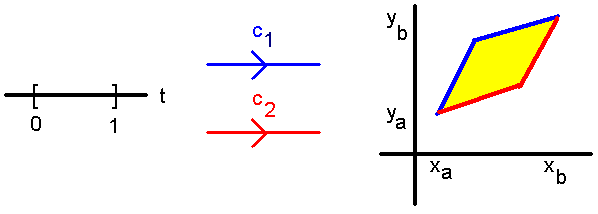
\includegraphics[scale=.5]{questao1}
		\end{center}

		A figura acima aproxima as imagens por poligonais, mas sem perda de generalidade suponha aplica\c{c}\~oes de classe $C^\infty$. Seja $\omega$ uma $1$-forma em $\mathbb{R}^2$.

		\begin{align}
			\omega &= u(x,y) \,\mathrm{d}x + v(x,y) \,\mathrm{d}y \\
			u, v : \mathbb{R}^2 &\rightarrow \mathbb{R} \\
			c_i : [0, 1] &\rightarrow A \times B \subset \mathbb{R}^2, \forall i \in \{1, 2\} \\
			c_i(0) &= (x_a, y_a) \\
			c_i(1) &= (x_b, y_b) \\
			c_i(t) &= (x_i(t), y_i(t)) \\
			\forall c_1, \forall c_2, \,\mathrm{temos}\, \int_{c_1} \omega &= \int_{c_2} \omega \label{Sete}
		\end{align}

		Queremos mostrar que $\omega$ \'e exata, isto \'e, seja $\theta$ uma $0$-forma em $\mathbb{R}^2$.

		\begin{align}
			\theta &= f(x,y) \\
			f : \mathbb{R}^2 &\rightarrow \mathbb{R} \\
			\omega = \mathrm{d}\theta &= \frac{\partial f}{\partial x} \,\mathrm{d}x + \frac{\partial f}{\partial y} \,\mathrm{d}y
		\end{align}

		Ou seja, \'e necess\'ario que exista $f$ tal que

		\begin{align}
			u &= \frac{\partial f}{\partial x} , v = \frac{\partial f}{\partial y} \label{Onze}\\
			\mathrm{Mas}\, (\ref{Sete}) \Rightarrow \int_{c_1} \omega - \int_{c_2} \omega &= 0 \\
			c_1 - c_2 &= \partial R, \text{ regi\~ao amarela da figura} \\
			\oint_{\partial R} \omega &= 0
		\end{align}

		Pelo teorema de Stokes,

		\begin{align}
			\int_{R} \mathrm{d}\omega &= 0 \\
			\int_{R} \biggl( -\frac{\partial u}{\partial y} + \frac{\partial v}{\partial x} \biggl) \,\mathrm{d}x \wedge \mathrm{d}y &= 0
		\end{align}

		Qual \'e a fun\c{c}\~ao cuja integral se anula para qualquer regi\~ao $R$? A fun\c{c}\~ao identicamente nula.

		\begin{align}
			\frac{\partial v}{\partial x} &= \frac{\partial u}{\partial y}
		\end{align}

		Utilizamos os problemas$^{[1]}$ 3.34 e 2.21 (a) para construir $f$, com $g_1 = u, g_2 = v$:

		\begin{align}
			\mathrm{D}_1 g_2 &= \mathrm{D}_2 g_1 \\
			f(x,y) &= \int_0^x g_1(t,0) \,\mathrm{d}t + \int_0^y g_2(x,t) \,\mathrm{d}t \\
			\Leftrightarrow f(x,y) &= \int_0^x u(t,0) \,\mathrm{d}t + \int_0^y v(x,t) \,\mathrm{d}t \\
			\mathrm{D}_1 f &= g_1, \mathrm{D}_2 f = g_2 \Leftrightarrow (\ref{Onze}),
		\end{align}

		como quer\'iamos demonstrar.

		\begin{flushright}
		\end{flushright}

	\subsection{Quest\~ao 1.b}
		\begin{flushright}
		\end{flushright}

		Toda forma exata \'e fechada.

		\begin{align}
			\omega = \mathrm{d}\theta \Rightarrow \mathrm{d}\omega = \mathrm{d}(\mathrm{d}\theta) = \mathrm{d}^2\theta = 0
		\end{align}

		Entretanto, a rec\'iproca n\~ao \'e verdadeira. Constru\'imos o contra-exemplo abaixo.

		\begin{align}
			\omega : \mathbb{R}^2 - \{0\} &\rightarrow \Lambda^1(\mathbb{R}^2) \\
			\omega &= \frac{-y}{x^2 + y^2} \,\mathrm{d}x + \frac{x}{x^2 + y^2} \,\mathrm{d}y \\
			A &= \{(x,y) \in \mathbb{R}^2 ; x < 0\} \cup  \{(x,y) \in \mathbb{R}^2 ; x \ge 0, y \neq 0\} \subset \mathbb{R}^2 \\
			\theta : A &\rightarrow (0, 2\pi) \subset \mathbb{R} \\
			\theta(x,y) &= \left\{
				\begin{aligned}
					\arctan \frac{y}{x}&, x > 0, y > 0 \\
					\pi + \arctan \frac{y}{x}&, x < 0 \\
					2 \pi + \arctan \frac{y}{x}&, x > 0, y < 0 \\
					\frac{\pi}{2}&, x = 0, y > 0 \\
					\frac{3 \pi}{2}&, x = 0, y < 0
				\end{aligned}
			\right. \\
			\omega &= \mathrm{d}\theta\,\mathrm{em\,}A \\
			\text{Suponha a extens\~ao}\,\,\omega &= \mathrm{d}f, f : \mathbb{R}^2 - \{0\} \rightarrow \mathbb{R} \\
			\text{Ent\~ao}\,\,\frac{\partial f}{\partial x} &= \frac{\partial \theta}{\partial x}, \frac{\partial f}{\partial y} = \frac{\partial \theta}{\partial y} \\
			f &= \theta + k, k \in \mathbb{R} \text{ Quod Erat Absurdum}
		\end{align}

	\section{Quest\~ao 2}
		\begin{align}
			f(t) &= c_1^A(t) = \begin{bmatrix} f_1(t) = 1 + \cos(2\pi t) \\ f_2(t) = \sin(2\pi t) \end{bmatrix} \\
			g(t) &= c_\pi^A(t) = \begin{bmatrix} g_1(t) = 1 + \pi \cos(2\pi t) \\ g_2(t) = \pi \sin(2\pi t) \end{bmatrix} \\
			f, g: [0,1] \subset \mathbb{R} &\rightarrow \mathbb{R}^2 \\
			F &= \begin{bmatrix} F_{11} \ F_{12} \\ F_{21} \ F_{22} \end{bmatrix} \\
			F_{11}(x,y) &= - \frac{y}{(x - 1)^2 + y^2} \\
			F_{12}(x,y) &= + \frac{x - 1}{(x - 1)^2 + y^2} \\
			F_{21}(x,y) &= - \frac{y}{(x + 1)^2 + y^2} \\
			F_{22}(x,y) &= + \frac{x+1}{(x + 1)^2 + y^2} \\
			F_{ij} : \mathbb{R}^2 &\rightarrow \mathbb{R} \\
			\omega_A &= F_{11} \,\mathrm{d}x + F_{12} \,\mathrm{d}y \\
			\omega_B &= F_{21} \,\mathrm{d}x + F_{22} \,\mathrm{d}y \\
			\omega &= \omega_A - \omega_B \\
			\int_f \omega &= \int_f \omega_A - \int_f \omega_B = \int_f F_{11} \,\mathrm{d}x + \int_f F_{12} \,\mathrm{d}y - \int_f F_{21} \,\mathrm{d}x - \int_f F_{22} \,\mathrm{d}y \label{Quinze} \\
			\int_g \omega &= \int_g \omega_A - \int_g \omega_B = \int_g F_{11} \,\mathrm{d}x + \int_g F_{12} \,\mathrm{d}y - \int_g F_{21} \,\mathrm{d}x - \int_g F_{22} \,\mathrm{d}y \label{Dezesseis} \\
			\int_f F_{11} \,\mathrm{d}x &= \int_0^1 f^*(F_{11} \,\mathrm{d}x) = \int_0^1 (F_{11} \circ f) f^*(\mathrm{d}x) = \int_0^1 (F_{11} \circ f) \frac{\partial f_1}{\partial t}\,\mathrm{d}t = \\
			&= \int_0^1 F_{11} \begin{pmatrix} 1 + \cos(2\pi t) \\ \sin(2\pi t) \end{pmatrix} (- \sin (2\pi t)) 2\pi \,\mathrm{d}t \\
			&= + 2 \pi \int_0^1 \frac{\sin(2\pi t)}{\cos^2(2\pi t) + \sin^2(2\pi t)} \sin (2\pi t) \,\mathrm{d}t \\
			&= 2 \pi \int_0^1 \sin^2 (2\pi t) \,\mathrm{d}t \\
			\int_f F_{12} \,\mathrm{d}y &= \int_0^1 f^*(F_{12} \,\mathrm{d}y) = \int_0^1 (F_{12} \circ f) f^*(\mathrm{d}y) = \int_0^1 (F_{12} \circ f) \frac{\partial f_2}{\partial t}\,\mathrm{d}t = \\
			&= \int_0^1 F_{12} \begin{pmatrix} 1 + \cos(2\pi t) \\ \sin(2\pi t) \end{pmatrix} \cos (2\pi t) 2\pi \,\mathrm{d}t \\
			&= 2\pi \int_0^1 \frac{\cos(2\pi t)}{\cos^2(2\pi t) + \sin^2(2\pi t)} \cos (2\pi t) \,\mathrm{d}t \\
			&= 2 \pi \int_0^1 \cos^2 (2\pi t) \,\mathrm{d}t \\
			- \int_f F_{21} \,\mathrm{d}x &= - \int_0^1 f^*(F_{21} \,\mathrm{d}x) = - \int_0^1 (F_{21} \circ f) f^*(\mathrm{d}x) = + \int_0^1 (F_{21} \circ f) \sin (2\pi t) 2\pi \,\mathrm{d}t = \\
			&= - 2\pi \int_0^1 \frac{\sin(2\pi t)}{(2 + \cos(2\pi t))^2 + \sin^2(2\pi t)} \sin (2 \pi t) \,\mathrm{d}t \\
			&= - 2\pi \int_0^1 \frac{\sin^2(2\pi t)}{4 \cos(2\pi t) + 5} \,\mathrm{d}t
		\end{align}

		\begin{align}
			- \int_f F_{22} \,\mathrm{d}y &= - \int_0^1 f^*(F_{22} \,\mathrm{d}y) = - \int_0^1 (F_{22} \circ f) f^*(\mathrm{d}y) = - \int_0^1 (F_{22} \circ f) \cos (2\pi t) 2\pi \,\mathrm{d}t \\
			& = - 2\pi \int_0^1 \frac{2 + \cos(2\pi t)}{(2 + \cos(2\pi t))^2 + \sin^2(2\pi t)} \cos (2\pi t) \,\mathrm{d}t \\
			& = - 2\pi \int_0^1 \frac{2\cos(2\pi t) + \cos^2(2\pi t)}{4 \cos(2\pi t) + 5} \,\mathrm{d}t \\
			(\ref{Quinze}) \Rightarrow \int_f \omega &= 2\pi \int_0^1 \biggl[ \sin^2 (2\pi t) + \cos^2 (2\pi t) - \frac{\sin^2(2\pi t) + 2\cos(2\pi t) + \cos^2(2\pi t)}{4 \cos(2\pi t) + 5} \biggl] \,\mathrm{d}t \\
			&= 2\pi \int_0^1 \biggl[ 1 - \frac{2\cos(2\pi t) + 1}{4 \cos(2\pi t) + 5} \biggl] \,\mathrm{d}t \\
			&= 2\pi \int_0^1 \biggl[ 1 - \frac{1}{2} + \frac{3}{2}\frac{1}{4 \cos(2\pi t) + 5} \biggl] \,\mathrm{d}t \\
			&= \pi \int_0^1 \biggl[ 1 + 3\frac{1}{4 \cos(2\pi t) + 5} \biggl] \,\mathrm{d}t \\
			&= \pi + 3\pi \int_0^1 \frac{\mathrm{d}t}{4 \cos(2\pi t) + 5} = \pi + 3\pi \frac{1}{3} = 2 \pi \\
			\int_g F_{11} \,\mathrm{d}x &= \int_0^1 g^*(F_{11} \,\mathrm{d}x) = \int_0^1 (F_{11} \circ g) g^*(\mathrm{d}x) = \int_0^1 (F_{11} \circ g) \frac{\partial g_1}{\partial t}\,\mathrm{d}t = \\
			&= \int_0^1 F_{11} \begin{pmatrix} 1 + \pi \cos(2\pi t) \\ \pi \sin(2\pi t) \end{pmatrix} \pi (-\sin (2\pi t)) 2\pi \,\mathrm{d}t \\
			&= + 2\pi^2 \int_0^1 \frac{\pi \sin(2\pi t) }{\pi^2 \cos^2(2\pi t) + \pi^2 \sin^2(2\pi t) } \sin (2\pi t) \,\mathrm{d}t \\
			&= 2\pi \int_0^1 \sin^2(2\pi t) \,\mathrm{d}t \\
			\int_g F_{12} \,\mathrm{d}y &= \int_0^1 g^*(F_{12} \,\mathrm{d}y) = \int_0^1 (F_{12} \circ g) \frac{\partial g_2}{\partial t}\,\mathrm{d}t = \\
			&= \int_0^1 F_{12} \begin{pmatrix} 1 + \pi \cos(2\pi t) \\ \pi \sin(2\pi t) \end{pmatrix} \pi \cos(2\pi t) 2\pi \,\mathrm{d}t \\
			&= 2\pi^2 \int_0^1 \frac{\pi \cos(2\pi t)}{\pi^2 \cos^2(2\pi t) + \pi^2 \sin^2(2\pi t)} \cos(2\pi t) \,\mathrm{d}t \\
			&= 2\pi \int_0^1 \cos^2(2\pi t) \,\mathrm{d}t \\
			- \int_g F_{21} \,\mathrm{d}x &= - \int_0^1 g^*(F_{21} \,\mathrm{d}x) = - \int_0^1 (F_{21} \circ g) g^*(\mathrm{d}x) = - \int_0^1 (F_{21} \circ g) \pi (-\sin (2\pi t)) 2\pi \,\mathrm{d}t \\
			&= - 2\pi^2 \int_0^1 \frac{\pi \sin(2\pi t)}{(2 + \pi \cos(2\pi t))^2 + \pi^2 \sin^2(2\pi t)} \sin (2\pi t) \,\mathrm{d}t \\
			&= - 2\pi^2 \int_0^1 \frac{\pi \sin^2(2\pi t)}{4 + 4 \pi \cos(2\pi t) + \pi^2} \,\mathrm{d}t \\
			- \int_g F_{22} \,\mathrm{d}y &= - \int_0^1 g^*(F_{22} \,\mathrm{d}y) = - \int_0^1 (F_{22} \circ g) g^*(\mathrm{d}y) = - \int_0^1 (F_{22} \circ g) \pi \cos(2\pi t) 2\pi \,\mathrm{d}t \\
			&= - 2 \pi^2 \int_0^1 \frac{2 + \pi \cos(2\pi t)}{(2 + \pi \cos(2\pi t))^2 + \pi^2 \sin^2(2\pi t)} \cos(2\pi t) \,\mathrm{d}t \\
			&= - 2 \pi^2 \int_0^1 \frac{2\cos(2\pi t) + \pi \cos^2(2\pi t)}{4 + 4 \pi \cos(2\pi t) + \pi^2} \,\mathrm{d}t
		\end{align}

		\begin{align}
			(\ref{Dezesseis}) \Rightarrow \int_g \omega &= 2\pi \int_0^1 [ \sin^2 (2\pi t) + \cos^2 (2\pi t) ] \,\mathrm{d}t - 2\pi^2 \int_0^1 \frac{\pi \sin^2(2\pi t) + 2\cos(2\pi t) + \pi \cos^2(2\pi t)}{4 + 4 \pi \cos(2\pi t) + \pi^2} \,\mathrm{d}t \\
			&= 2\pi \int_0^1 \mathrm{d}t - 2\pi^2 \int_0^1 \frac{2\cos(2\pi t) + \pi}{4 \pi \cos(2\pi t) + \pi^2 + 4} \,\mathrm{d}t \\
			&= 2\pi - 2\pi^2 \int_0^1 \biggl[\frac{1}{2\pi} + \frac{\pi^2 - 4}{2\pi} \frac{1}{4 \pi \cos(2\pi t) + \pi^2 + 4} \biggl] \,\mathrm{d}t \\
			&= 2\pi - \pi \int_0^1 \mathrm{d}t - \pi (\pi^2-4) \int_0^1 \frac{\mathrm{d}t}{4 \pi \cos(2\pi t) + \pi^2 + 4} \\
			&= 2\pi - \pi - \pi (\pi^2-4) \frac{1}{\pi^2 - 4} = 0
		\end{align}

		\begin{flushright}
		\end{flushright}

	\section{Quest\~ao 3}
		\begin{center}
		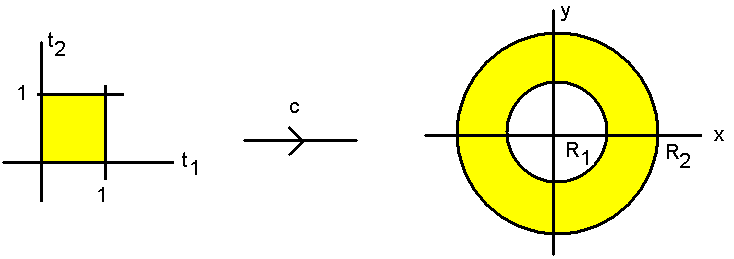
\includegraphics[scale=.5]{questao3}
		\end{center}

		Na imagem de $c$, $t_1$ representa o raio, $t_2$ representa o \^angulo. Suponha $R_2 > R_1$.

		\begin{align}
			c_{R,n}(t) &= \begin{bmatrix} R \cos(2\pi nt) \\ R \sin(2\pi nt) \end{bmatrix} \\
			R &> 0, n \neq 0 \\
			c_{R,n} : [0,1] &\rightarrow \mathbb{R}^2 - \{0\} \\
			\exists c &\in C^\infty( (0,1)^2 \rightarrow \mathbb{R}^2 - \{0\} ) ; \partial c = c_{R_1,n} - c_{R_2,n} \\
			c(t_1, t_2) &= \begin{bmatrix} \rho(t_1) \cos(2\pi nt_2) \\ \rho(t_1) \sin(2\pi nt_2) \end{bmatrix} \mathrm{\,tal\,que\,} \rho(0) = R_1 , \rho(1) = R_2 \\
			\rho(t_1) &= a t_1 + b \Rightarrow b = R_1, a = \frac{R_2 - R_1}{1 - 0} \\
			c(t_1, t_2) &= \begin{bmatrix} [(R_2 - R_1) t_1 + R_1] \cos(2\pi nt_2) \\ [(R_2 - R_1) t_1 + R_1]  \sin(2\pi nt_2) \end{bmatrix}
		\end{align}

		O per\'iodo de $f(x) = \cos(a x) = f(x + T)$ ou $g(x) = \sin (a x) = g(x + T)$ \'e:

		\begin{align}
			|a| T = 2 \pi \Rightarrow T = \frac{2 \pi}{|a|}
		\end{align}

		em que $T$ equivale ao n\'umero de voltas sobre $S^1$ quando $x$ percorre o dom\'inio $[0, 1] \subset \mathbb{R}$.

		Logo, o per\'iodo de $c_{R,n}$ \'e

		\begin{align}
			\frac{2 \pi}{|2 \pi n|} = \frac{1}{|n|}
		\end{align}

		Portanto, o bordo de $c$ d\'a $|n|$ voltas sobre o c\'irculo maior e $|n|$ voltas sobre o c\'irculo menor.

		Seja $m \neq n$. Sem perda de generalidade, suponhamos dois c\'irculos completos: $|m|, |n| \ge 1$.

		Podemos variar o per\'iodo com o raio:

		\begin{align}
			\partial C &= c_{R_1,m} - c_{R_2,n} \\
			C(t_1, t_2) &= \begin{bmatrix} [(R_2 - R_1) t_1 + R_1] \cos(2\pi t_2 N(t_1)) \\ [(R_2 - R_1) t_1 + R_1]  \sin(2\pi t_2 N(t_1)) \end{bmatrix} \mathrm{\,tal\,que\,} N(0) = m, N(1) = n \\
			N(t_1) &= A t_1 + B \Rightarrow B = m, A = \frac{n - m}{1 - 0} \\
			C(t_1, t_2) &= \begin{bmatrix} [(R_2 - R_1) t_1 + R_1] \cos(2\pi t_2 ((n - m) t_1 + m)) \\ [(R_2 - R_1) t_1 + R_1]  \sin(2\pi t_2 ((n - m) t_1 + m)) \end{bmatrix}
		\end{align}

		O bordo de $C$ d\'a $|n|$ voltas sobre o c\'irculo maior e $|m|$ voltas sobre o c\'irculo menor.

		Portanto, por constru\c{c}\~ao, sim, podemos dizer o mesmo:

		\begin{align}
			\exists C &\in C^\infty( (0,1)^2 \rightarrow \mathbb{R}^2 - \{0\} ) ; \partial C = c_{R_1,m} - c_{R_2,n}
		\end{align}

	\section{Refer\^encia}

		$[1]$ SPIVAK, M. Calculus on Manifolds. Addisson-Wesley Publishing Company, 1965
\end{document}
